%%% LaTeX Template: Two column article
%%%
%%% Source: http://www.howtotex.com/
%%% Feel free to distribute this template, but please keep to referal to http://www.howtotex.com/ here.
%%% Date: February 2011

%%% Preamble
\documentclass[	DIV=calc,%
							paper=a4,%
							fontsize=12pt,%
							onecolumn]{scrartcl}	 					% KOMA-article class

\usepackage{lipsum}													% Package to create dummy text
\usepackage[brazil]{babel}										% English language/hyphenation
\usepackage[protrusion=true,expansion=true]{microtype}				% Better typography
\usepackage{amsmath,amsfonts,amsthm}					% Math packages
\usepackage[pdftex]{graphicx}									% Enable pdflatex
\usepackage[svgnames]{xcolor}									% Enabling colors by their 'svgnames'
\usepackage[hang, small,labelfont=bf,up,textfont=it,up]{caption}	% Custom captions under/above floats
\usepackage{epstopdf}												% Converts .eps to .pdf
\usepackage{subfig}													% Subfigures
\usepackage{booktabs}												% Nicer tables
\usepackage{fix-cm}													% Custom fontsizes
\usepackage[utf8]{inputenc}
\usepackage[top=2.5cm, bottom=2.5cm, left=2.5cm, right=2.5cm]{geometry}
\usepackage[ddmmyyyy]{datetime}
\usepackage{float}
	\renewcommand\tablename{Tabela}
	\renewcommand\figurename{Figura}
 
 

 
%%% Custom sectioning (sectsty package)
\usepackage{sectsty}													% Custom sectioning (see below)
\allsectionsfont{%															% Change font of al section commands
	\usefont{OT1}{phv}{b}{n}%										% bch-b-n: CharterBT-Bold font
	}

\sectionfont{%																% Change font of \section command
	\usefont{OT1}{phv}{b}{n}%										% bch-b-n: CharterBT-Bold font
	}



%%% Headers and footers
\usepackage{fancyhdr}												% Needed to define custom headers/footers
	\pagestyle{fancy}														% Enabling the custom headers/footers
\usepackage{lastpage}	

% Header (empty)
\lhead{}
\chead{}
\rhead{}
% Footer (you may change this to your own needs)

%% ====================================
%% ====================================
%% mude o rodape  do projeto
%% ====================================
%% ====================================

\lfoot{\footnotesize \texttt{Planejamento e Projeto de Cabeamento Estruturado} }

\cfoot{}
\rfoot{\footnotesize página \thepage\ de \pageref{LastPage}}	% "Page 1 of 2"
\renewcommand{\headrulewidth}{0.0pt}
\renewcommand{\footrulewidth}{0.4pt}



%%% Creating an initial of the very first character of the content
\usepackage{lettrine}
\newcommand{\initial}[1]{%
     \lettrine[lines=3,lhang=0.3,nindent=0em]{
     				\color{DarkGoldenrod}
     				{\textsf{#1}}}{}}



%%% Title, author and date metadata
\usepackage{titling}															% For custom titles

\newcommand{\HorRule}{\color{DarkGoldenrod}%			% Creating a horizontal rule
									  	\rule{\linewidth}{1pt}%
										}

\pretitle{\vspace{-30pt} \begin{flushleft} \HorRule 
				\fontsize{50}{50} \usefont{OT1}{phv}{b}{n} \color{blue} \selectfont 
				}

%% ====================================
%% ====================================
%% mude o titulo  do projeto
%% ====================================
%% ====================================

\title{Planejamento e Projeto de Cabeamento Estruturado}					% Title of your article goes here

%% ====================================



\posttitle{\par\end{flushleft}\vskip 0.5em}

\preauthor{\begin{flushleft}
					\large \lineskip 0.5em \usefont{OT1}{phv}{b}{sl} \color{black}}
\author{Lucas Vinicius Timm}  	% Author name goes here


\postauthor{\footnotesize \usefont{OT1}{phv}{m}{sl} \color{Black} 
					\\Universidade Tecnológica Federal do Paraná - Câmpus Cornélio Procópio 								% Institution of author
					\par\end{flushleft}\HorRule}

\date{}																				% No date




%%% Begin document
\begin{document}
\maketitle
\thispagestyle{fancy} 	
\thispagestyle{empty}		% Enabling the custom headers/footers for the first page 
% The first character should be within \initial{}




%% ====================================
%% ====================================
%% mude o resumo  do projeto
%% ====================================
%% ====================================
\initial{E}\textbf{ste trabalho mostra uma visão sobre cabeamento estruturado das redes de
computadores. A rede atual foi analisada e, posteriormente, uma rede de cabeamento
estruturado foi proposta para as dependências do edificio San Luigi, com o intuito de
melhorar a estrutura da rede instalada, permitindo maior organização, flexibilidade e
integração. Serão apresentados os projetos lógico e físico com base nas plantas baixas apresentadas pela administração do condomínio.}

%% ====================================
\begin{figure}
	\centering
	
\includegraphics{utfpr}
\end{figure}

\vspace{3cm}
\centerline{\textit{\textbf{\today}}}

\clearpage
    \renewcommand*\listfigurename{Lista de figuras}
\listoffigures

\renewcommand*\listtablename{Lista de tabelas}
\listoftables




\clearpage
\renewcommand{\contentsname}{Sumário}
\tableofcontents
\clearpage

%% ====================================
%% ====================================
%% Inicio do texto
%% ====================================
%% ====================================
\section{Introdução}
{\raggedright O projeto se propõe, através de uma rede de computadores (servidores, esquipamentos de rede e cabeamento estruturado), prover conectividade entre os mesmos, permitindo o intercâmbio de informações entre estes equipamentos de uma forma segura e rápida. Inerente a isto, serão utilizados recursos tecnológicos de informática a fim de implantar um ambiente estável, definir infra-estruturas, padrões que possam ter escalabilidade, grande vida útil através de excelente custo benefício.}

\section{Ambiente}

{\raggedright O condomínio San Luigi, sito a Rua Ângelo Donin, Jardim Concordia, Toledo - PR, possui três andares que totalizam 10 salas comerciais. Tais salas terão tratamento diferenciado quanto à
implantação da infraestrutura de redes, o qual levará em conta: o tipo de negócio a ser
praticado em cada uma, o tamanho da empresa, a quantidade de funcionários e um plano de expansão.
}

\begin{figure}[H]
  \centering
  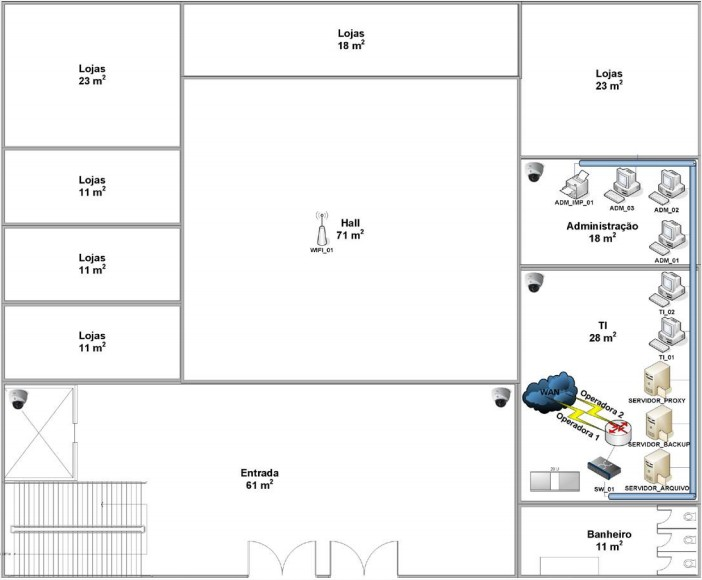
\includegraphics[width=\textwidth]{terreo} 
  \caption{PISO TÉRREO (ADMINISTRAÇÃO, HALL E TI)}
  \label{fig:methodology}
\end{figure}

\begin{figure}[H]
  \centering
  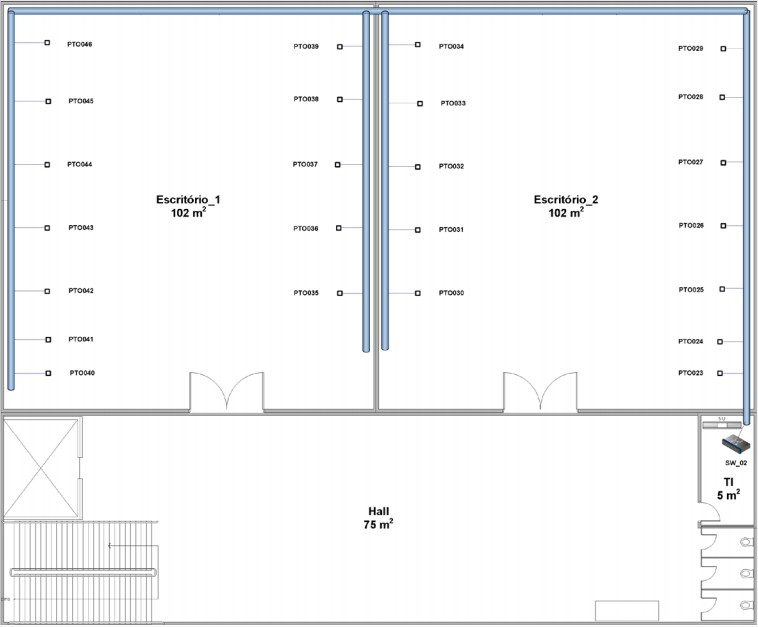
\includegraphics[width=\textwidth]{piso1} 
  \caption{1º ANDAR (ESCRITÓRIOS 1 E 2)}
  \label{fig:methodology}
\end{figure}

\begin{figure}[H]
  \centering
  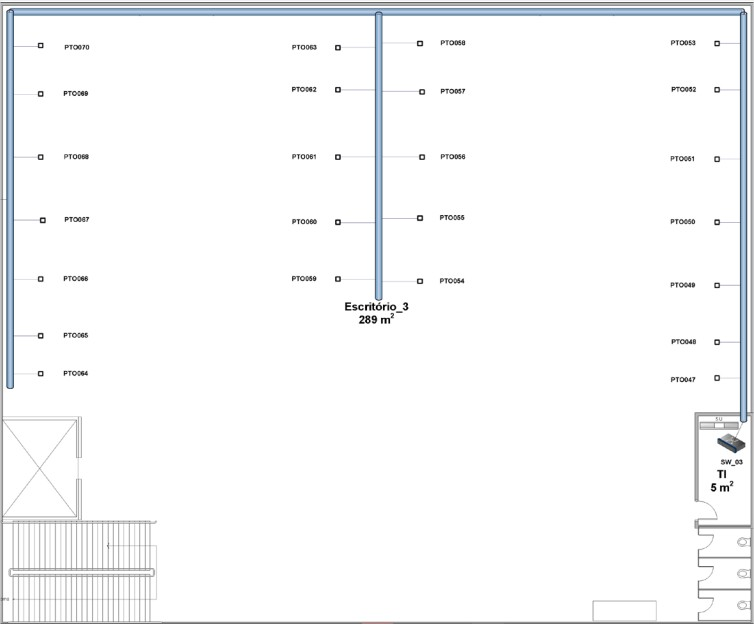
\includegraphics[width=\textwidth]{piso2} 
  \caption{2º ANDAR (ESCRITÓRIO 3)}
  \label{fig:methodology}
\end{figure}


\section{Cabeamento Estruturado}
{\raggedright Serão tratados neste item o projeto da rede física de cada andar, de uma forma isolada.
Além disso, as salas de suporte e a sala de controle de TI terão planejamento à parte no projeto. Em todos os andares serão instaladas eletrocalhas na parte superior para passagem do cabeamento estruturado da rede. 
A cada ponto de rede do patch panel terá um cabo de rede ( patch cord) de 1,5 metro para fazer a ligação ao switch.
}

\subsection{Térreo}
{\raggedright Conforme a figura 4, serão instaladas eletrocalhas para a passagem do cabeamento de
rede no primeiro andar para a instalação de 2 pontos de rede por sala, totalizando 14
pontos de rede nas salas. Além disto, serão instaladas 3 cameras e 1 ponto de acesso sem
fio neste andar. Desta forma, serão necessários 17 pontos para este andar. Todos estes
pontos serão levados a sala de operações e conectados a um patch panel no rack central.
O mapeamento dos pontos no patch panel será anexado a este projeto.
Considerando que serão utilizados patch panel de 24 porta cada, será necessário para este pavimento apenas 1 unidade.}

\begin{figure}[H]
  \centering
  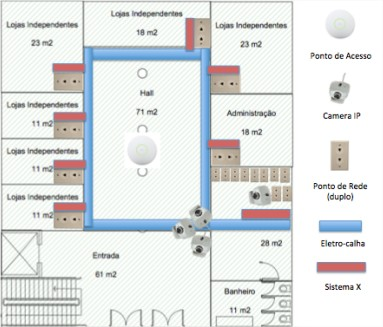
\includegraphics[width=\textwidth]{terro1} 
  \caption{Cabeamento Estruturado}
  \label{fig:methodology}
\end{figure}

\subsection{Sala de Operações}
{\raggedright Neste ambiente ficará localizada toda a infraestrutura de TI do condomínio. A partir dela
chegará o link de internet do provedor de acesso a internet, sairão as ligações aos outros andares bem como todos o cabeamento do primeiro pavimento.
Conforme descrito anteriormente, para o primeiro pavimento será necessária a utilização de 1 patch panel para os pontos deste andar. Tais pontos serão ligados no rack a um switch de rede Gigabit 10/100/1000 por cabos de rede categoria 6 ou 5e.
Além disto, serão utilizados 6 servidores que utilizaram 3 pontos de rede cada, 2
nobreaks cada um utilizando 1 ponto de rede e 1 câmera IP para monitoramento específico
desta sala. No total, para a infraestrutura dos servidores serão utilizados 21 pontos. Para
a ligação entre os pavimentos (térreo para 2 andar e térreo para 3 andar) serão utilizados
links de fibra óptica direta e também 2 links (1 para cada pavimento) de cabo de rede
categoria 5e.
No total serão utilizados dois patch panels de 24 portas cada, um exclusivo para
o primeiro pavimento e outro exclusivo para a sala de operações.
Para este andar serão necessários 80 metros de eletro calha de 0,30 cm de largura,
10 metros de sistema X de 0,20cm de largura, 18 espelhos duplos de rede e 8 espelhos
simples de rede.
Serão ainda utilizadas 2 (duas) caixas de cabo de rede categoria 5e com 305
metros cada. A previsão de gasto para este andar é de 450 metros. A eventual sobra
deste cabeamento ficará disponível para eventuais alterações futuras e para ligar os demais
pavimentos ao térreo. Esta ligação via cabo cat 5e será utilizada apenas como redundância
na rede e não link principal.
Por fim será feito cabeamento entre os andares por meio de fibra óptica de 15
metros cada (Multimodo).
}
\subsection{Segundo Pavimento}
{\raggedright Conforme a figura 6.2, no segundo pavimento também serão instaladas eletrocalhas para a
passagem do cabeamento de rede. No total serão ligados 20 pontos de rede por escritório
(escritório 1 e escritório 2) totalizando 40 pontos de rede neste andar. Além disto, cada
escritório terá monitoramento por 4 câmeras de vigilância, 1 ponto de acesso à rede sem
fio e na área comum ”hall” do segundo paviemento serão instalados 1 ponto de acesso a
rede sem fio e 1 camera IP. No total serão instalados 52 pontos neste pavimento.
Todos estes pontos serão levados a sala de TI deste mesmo pavimento e conectados
a um patch panel no rack 2.
Considerando que serã o utilizados patch panels de 24 portas cada, será necessário
para estes pontos 3 unidades.
Para este andar serão necessários 250 metros de eletrocalha de 0,30 cm de largura,
30 metros de sistema X de 0,20cm de largura, 22 espelhos duplos de rede e 8 espelhos
simples de rede.
Serão ainda utilizadas 4 (quatro) caixas de cabo de rede categoria 5e com 305
metros cada. A previsão de gasto para este andar é de 1150 metros.
}
\begin{figure}[H]
  \centering
  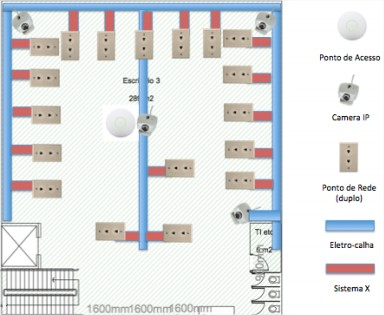
\includegraphics[width=\textwidth]{piso22} 
  \caption{Cabeamento Estruturado}
  \label{fig:methodology}
\end{figure}

\subsection{Terceiro Pavimento}
{\raggedright Conforme a figura 6.3 no terceiro pavimento serão instaladas eletrocalhas para a passagem
do cabeamento de rede. No total serão ligados 36 pontos de rede para o único escritório
deste pavimento. Além disto, também serão instaladas 4 câmeras de vigilância e 1 ponto
de acesso à rede sem fio, totalizando 41 pontos.
}
\begin{figure}[H]
  \centering
  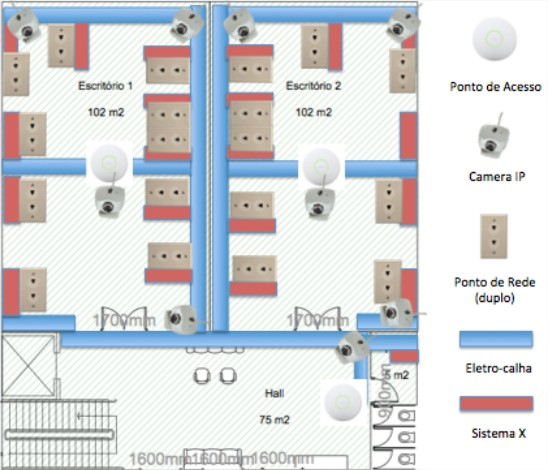
\includegraphics[width=\textwidth]{piso33} 
  \caption{Cabeamento Estruturado}
  \label{fig:methodology}
\end{figure}

\subsection{Orçamento Cabeamento Estruturado}
{\raggedright Conforme a Tabela 1 e Tabela 2 são as quantidade e gastos para implementar o cabeamento estuturado no Edifício são Luigi.
}
\begin{table}[H]
\centering
\caption{Quantidade Cabeamento Estrututado}
\label{my-label}
\begin{tabular}{lllll}
Andar                   & 1  & 2   & 3   & Total \\
Eletrocalha             & 80 & 250 & 350 & 680   \\
Sistama X               & 10 & 30  & 50  & 90    \\
Espelho RJ 45 (Duplo)   & 17 & 22  & 19  & 58    \\
Espelho RJ 45 (Simples) & 5  & 8   & 3   & 16    \\
Cat 5e 305m             & 2  & 4   & 12  & 18    \\
Pach Panel              & 2  & 3   & 2   & 7     \\
Pach Cord               & 39 & 40  & 41  & 120   \\
Fibra Optica (15m)      & 2  & 0   & 0   & 2    
\end{tabular}
\end{table}
\begin{table}[H]
\centering
\caption{Valor Cabeamento Estrututado}
\label{my-label}
\begin{tabular}{|l|l|l|l|}
\hline
\textbf{Andar}          & \textbf{Quantidade} & \textbf{Preço} & \textbf{Total} \\ \hline
Eletrocalha             & 680                 & 18             & 12240          \\ \hline
Sistama X               & 90                  & 6              & 540            \\ \hline
Espelho RJ 45 (Duplo)   & 58                  & 12             & 696            \\ \hline
Espelho RJ 45 (Simples) & 16                  & 8              & 128            \\ \hline
Cat 5e 305m             & 7                   & 90             & 630            \\ \hline
Pach Panel              & 120                 & 3,9            & 468            \\ \hline
Pach Cord               & 39                  & 40             & 469            \\ \hline
Fibra Optica (15m)      & 2                   & 195            & 390            \\ \hline
\textbf{Total}          &                     &                & \textbf{17792} \\ \hline
\end{tabular}
\end{table}

\section{Planta da Rede Lógica}
\subsection{Topologia da Rede}

{\raggedright Consideramos a utilização de um cabeamento para cada andar do edifício (cabeamento
horizontal) que se conectará ao backbone (cabeamento central). Em cada andar existirá uma sala
para onde convergem todos os cabos do andar, interligando os dispositivos da rede a um Patch
Panel, que será ligado ao backbone central. No térreo do edifício teremos um switch que atua
como um ponto central da rede num formato de estrela.
Em cada andar será utilizado um switch para centralizar os dispositivos (SW02 e SW03).
Estes switches serão conectados num Switch central (SW01) que fará a verificação de destino
dos pacotes e em caso de necessidade irá repassar os pacotes para o roteador que fará acesso
externo (WAN-Internet). O roteador, por sua vez, será contratado junto com o plano de acesso da
operadora, sendo de sua responsabilidade a configuração e manutenção do equipamento.
A rede será segmentada por sub-redes, de forma a agrupar os dispositivos de mesmo nível,
restringir o acesso não autorizado e segmentar o domínio de colisão dos pacotes em trânsito.
}
\subsection{Diagrama do Projeto Lógico}
\begin{figure}[H]
  \centering
  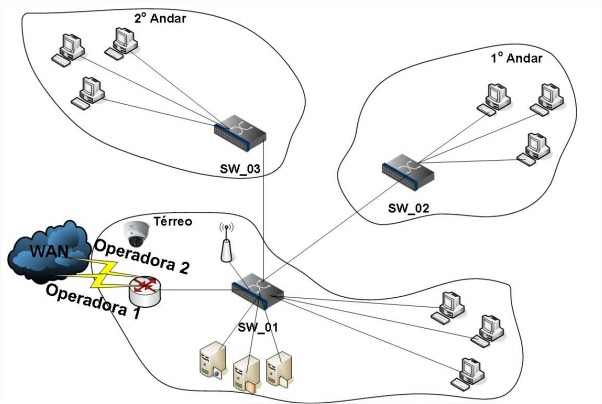
\includegraphics[width=\textwidth]{projeto_logico} 
  \caption{Cabeamento Estruturado}
  \label{fig:methodology}
\end{figure}

\subsection{Nomenclaturas}
{\raggedright Para facilitar a identificação dos componentes no projetos, criamo a seguinte regras:

• SW-XX = Switches de rede de 00 a 99;

• WIFI-XX = Roteadores sem fio (APs) de 00 a 99;

• Operadora-X = Links de Internet redundantes das operadoras de 0 a 9;

• PTOXXX = Pontos de rede distribuídos ao longo do prédio;

• ADM-XX = Estações de trabalho da administração do condomínio;

• ADM-IMP-XX = Impressoras de rede da administração do condomínio;

• TI-XX = Estações de trabalho do departamento de tecnologia da informação;
}

\subsection{Endereçamento}
{\raggedright A rede será segmentada por sub-redes, de forma a agrupar os dispositivos de mesmo nível,
restringir o acesso não autorizado e segmentar o domínio de colisão dos pacotes em trânsito.
Nesta seção do projeto, determinamos o endereço de rede a ser utilizado, a máscara de sub rede,
as sub-redes, a faixa de IPs. Não faremos a identificação individual dos IPs, pois teremos 20
sub-redes para distribuirmos a medida em que as salas forem ativadas.
}
{\raggedright Serão 20 subredes com 62 hosts possíveis em cada:}
\begin{table}[H]
\centering
\caption{Endereçamento IP}
\label{my-label}
\begin{tabular}{@{}|l|l|l|l|l|l|l|l|@{}}
\toprule
\multicolumn{1}{|c|}{ID} & \multicolumn{1}{c|}{\textbf{END.REDE}} & \multicolumn{1}{c|}{\textbf{\begin{tabular}[c]{@{}c@{}}END.\\ BROAD.\end{tabular}}} & \multicolumn{1}{c|}{\textbf{\begin{tabular}[c]{@{}c@{}}PRIM. \\ MAQ.\end{tabular}}} & \multicolumn{1}{c|}{\textbf{\begin{tabular}[c]{@{}c@{}}ULT. \\ MAQ.\end{tabular}}} & \textbf{\begin{tabular}[c]{@{}l@{}}SUB \\ REDE\end{tabular}} & \textbf{\begin{tabular}[c]{@{}l@{}}BITS \\ HOSTS\end{tabular}} & \textbf{\begin{tabular}[c]{@{}l@{}}TOTAL \\ HOST\end{tabular}} \\ \midrule
\textbf{1}               & 105.3.128.0                            & 105.3.128.63                                                                        & 105.3.128.1                                                                         & 105.3.128.62                                                                       & 26                                                           & 6                                                              & 62                                                             \\ \midrule
\textbf{2}               & 105.3.128.64                           & 105.3.128.127                                                                       & 105.3.128.65                                                                        & 105.3.128.126                                                                      & 26                                                           & 6                                                              & 62                                                             \\ \midrule
\textbf{3}               & 105.3.128.128                          & 105.3.128.191                                                                       & 105.3.128.129                                                                       & 105.3.128.190                                                                      & 26                                                           & 6                                                              & 62                                                             \\ \midrule
\textbf{4}               & 105.3.128.192                          & 105.3.128.255                                                                       & 105.3.128.193                                                                       & 105.3.128.254                                                                      & 26                                                           & 6                                                              & 62                                                             \\ \midrule
\textbf{5}               & 105.3.129.0                            & 105.3.129.63                                                                        & 105.3.129.1                                                                         & 105.3.129.62                                                                       & 26                                                           & 6                                                              & 62                                                             \\ \midrule
\textbf{6}               & 105.3.129.64                           & 105.3.129.127                                                                       & 105.3.129.65                                                                        & 105.3.129.126                                                                      & 26                                                           & 6                                                              & 62                                                             \\ \midrule
\textbf{7}               & 105.3.129.128                          & 105.3.129.191                                                                       & 105.3.129.129                                                                       & 105.3.129.190                                                                      & 26                                                           & 6                                                              & 62                                                             \\ \midrule
\textbf{8}               & 105.3.129.192                          & 105.3.129.255                                                                       & 105.3.129.193                                                                       & 105.3.129.254                                                                      & 26                                                           & 6                                                              & 62                                                             \\ \midrule
\textbf{9}               & 105.3.130.0                            & 105.3.130.63                                                                        & 105.3.130.1                                                                         & 105.3.130.62                                                                       & 26                                                           & 6                                                              & 62                                                             \\ \midrule
\textbf{10}              & 105.3.130.64                           & 105.3.130.127                                                                       & 105.3.130.65                                                                        & 105.3.130.126                                                                      & 26                                                           & 6                                                              & 62                                                             \\ \midrule
\textbf{11}              & 105.3.130.128                          & 105.3.130.191                                                                       & 105.3.130.129                                                                       & 105.3.130.190                                                                      & 26                                                           & 6                                                              & 62                                                             \\ \midrule
\textbf{12}              & 105.3.130.192                          & 105.3.130.255                                                                       & 105.3.130.193                                                                       & 105.3.130.254                                                                      & 26                                                           & 6                                                              & 62                                                             \\ \midrule
\textbf{13}              & 105.3.131.0                            & 105.3.131.63                                                                        & 105.3.131.1                                                                         & 105.3.131.62                                                                       & 26                                                           & 6                                                              & 62                                                             \\ \midrule
\textbf{14}              & 105.3.131.64                           & 105.3.131.127                                                                       & 105.3.131.65                                                                        & 105.3.131.126                                                                      & 26                                                           & 6                                                              & 62                                                             \\ \midrule
\textbf{15}              & 105.3.131.128                          & 105.3.131.191                                                                       & 105.3.131.129                                                                       & 105.3.131.190                                                                      & 26                                                           & 6                                                              & 62                                                             \\ \midrule
\textbf{16}              & 105.3.131.192                          & 105.3.131.255                                                                       & 105.3.131.193                                                                       & 105.3.131.254                                                                      & 26                                                           & 6                                                              & 62                                                             \\ \midrule
\textbf{17}              & 105.3.132.0                            & 105.3.132.63                                                                        & 105.3.132.1                                                                         & 105.3.132.62                                                                       & 26                                                           & 6                                                              & 62                                                             \\ \midrule
\textbf{18}              & 105.3.132.64                           & 105.3.132.127                                                                       & 105.3.132.65                                                                        & 105.3.132.126                                                                      & 26                                                           & 6                                                              & 62                                                             \\ \midrule
\textbf{19}              & 105.3.132.128                          & 105.3.132.191                                                                       & 105.3.132.129                                                                       & 105.3.132.190                                                                      & 26                                                           & 6                                                              & 62                                                             \\ \midrule
\textbf{20}              & 105.3.132.192                          & 105.3.132.255                                                                       & 105.3.132.193                                                                       & 105.3.132.254                                                                      & 26                                                           & 6                                                              & 62                                                             \\ \bottomrule
\end{tabular}
\end{table}

\subsection{Segurança}
{\raggedright  O acesso à rede compartilhada do condomínio se dará por meio do cadastro e liberação de
endereço MAC das placas de rede dos clientes, para que haja controle e rastreabilidade das
conexões, que a princípio ficarão ativas e com os endereços IP, dentro de cada faixa, concedido
automaticamente via DHCP do servidor Proxy.
Em relação à segurança de acesso aos sites, o servidor Proxy conterá regras simplificadas
bloqueios a sites indesejados e controle de portas, evitando assim, que a rede do condomínio seja
invadida por intrusos.
No quesito compartilhamento de arquivos, o serviço ficará disponível para os clientes do
condomínio registrados no domínio SAOLUIGI-XX, onde XX significa o domínio de determinado
escritório, para aumentar a segurança e permitir o uso de perfis bem definidos para cada empresa
contratante. Estes compartilhamentos serão acessados somente via clientes registrados por MAC
na rede interna e com login e senha válida no domínio SAOLUIGI-XX. O condomínio oferecerá, para os clientes que utilizam o serviço de compartilhamento de arquivos, um sistema de backup online exclusivo. O serviço roda todos os dias, à 00h00min da manhã, inclusive nos feriados e finais de semana. A recuperação pode ser feita mediante solicitação à administração do condomínio, que abrirá uma aquisição junto à equipe de TI local.
}
\section{Projeto Rede Fisica}
\subsection{Topologia}
{\raggedright Este projeto de rede será utilizado como padrão para as empresas que se instalarem no condomínio, prevendo a expansão das redes existentes. Cada escritório possui a capacidade para abrigar cerca de 10 funcionários, exceto o segundo andar, que tem o dobro do tamanho, logo pode ser ocupado por até 20 funcionários. O piso térreo possui lojas que não fazem uso da rede do condomínio, mas engloba a administração e a sala de TI, onde ficam os servidores. São três pisos ao todo, cada um com 289m de área útil.Basicamente será utilizado o padrão modelo OSI para funcionamento de redes locais. Dentre
os materiais e equipamentos serão usados cabos UTP Categoria 6 para conexão dos equipamentos, LAN Gigabit, equipamentos de alta confiabilidade e protocolo TCP/IP. O acesso a rede externa (WAN) será provido por duas operadoras de telefonia, por meios físicos distintos (fibra ótica e WiMax), para garantirmos a redundância do acesso, seja por meio físico ou contratual. As operadoras escolhidas ficarão responsáveis pela instalação, configuração e manutenção dos equipamentos com SLA mínimo de duas horas, 24 x 7. A largura de banda definida será de 10Mbps, podendo crescer a medida que for necessária. Todo o tráfego externo será conduzido pelo servidor Proxy localizado no departamento de TI do condomínio. 
}
\subsection{Mapa da Rede}
{\raggedright A imagem a seguir ilustra a distribuição física dos equipamentos, quanto a sua disposição:  }

\begin{figure}[H]
  \centering
  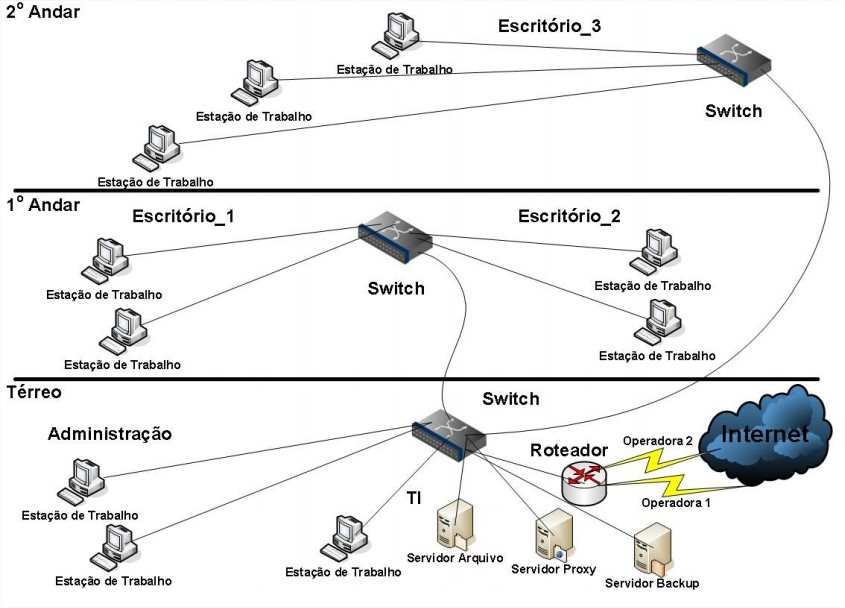
\includegraphics[width=\textwidth]{mapa_rede} 
  \caption{Cabeamento Estruturado}
  \label{fig:methodology}
\end{figure}

\subsection{Cabeamento Estruturado}
{\raggedright Documentamos, a seguir, as conexões Porta Ponto dos respectivos equipamentos de rede:
}
\begin{figure}[H]
  \centering
  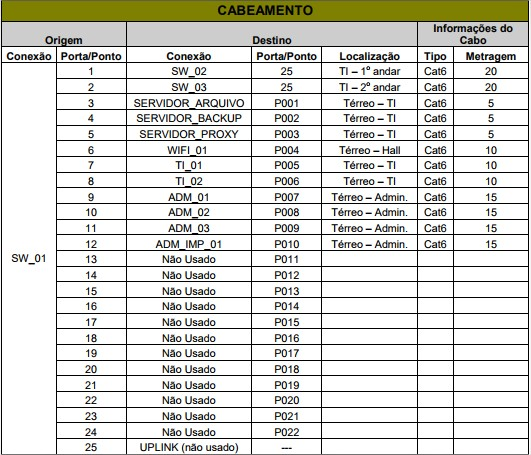
\includegraphics[width=\textwidth]{sw-01} 
  \caption{Térreo Switch 01}
  \label{fig:methodology}
\end{figure}
\begin{figure}[H]
  \centering
  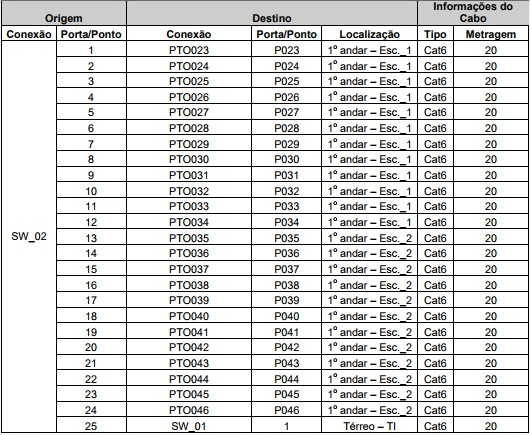
\includegraphics[width=\textwidth]{sw-02} 
  \caption{Piso 1 Switch 02}
  \label{fig:methodology}
\end{figure}
\begin{figure}[H]
  \centering
  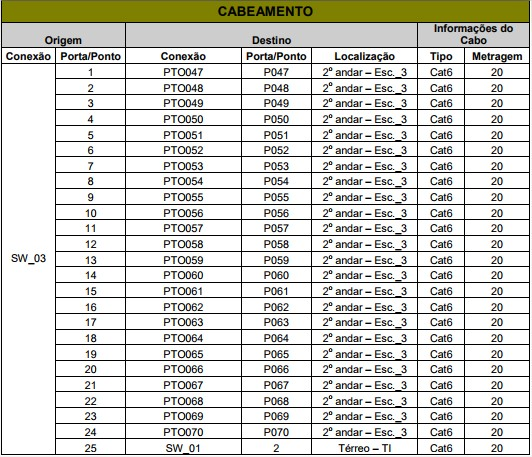
\includegraphics[width=\textwidth]{sw-03} 
  \caption{Piso 2 Switch 03}
  \label{fig:methodology}
\end{figure}

{\raggedright Obs.: apesar dos swtiches envolvidos neste projeto serem de 24 portas, a porta 25 existente
na tabela representa a porta extra contida nestes equipamentos com a finalidade de UPLINK, isto
é, para permitir o cascateamento das conexões do switch para outro mais central, sem comprometer o desempenho das demais 24 portas utilizadas. 
}
\subsection{Certificação}

{\raggedright  Essa certificação do cabeamento deve ser realizada antes da rede ser ativada, pois, após a ativação da rede, torna-se muito difícil localizar a causa de um eventual defeito que possa surgir. Além disso, existe o inconveniente de desativar toda a rede ou parte dela.

A certificação dessa rede envolve uma série de testes que avaliam os parâmetros do cabeamento. Na prática, esses parâmetros demonstram a qualidade geral do cabeamento de uma rede local. Podendo garantir um ótimo desempenho para o qual a rede foi planejada.

Para efetuar-se a certificação, utilizamos um equipamento específico devidamente calibrado capaz de detectar possíveis falhas seguindo as normas TIA/EIA 568B. Após toda análise é emitido um relatório de testes, com o resultado do teste e dos parâmetros avaliados; Esses relatórios são úteis para anexar a documentação que deve acompanhar o projeto da instalação. 
O que será analizado:

Comprimento do Cabo;

Mapeamento dos Condutores;

Atenuação;

Paradiafonia;

Impedância Característica;

Resistência do Cabo;

EL-FEXT, Return Loss e Skew Delay;

}
\section{Orçamento}
{\raggedright Seguem os orçamentos finais obtidos após as coletas de preços junto aos fornecedores de materiais e serviços.
}
\begin{table}[H]
\centering
\caption{Equipamentos e Periféricos}                                                                     
\label{my-label}
\begin{tabular}{|c|c|c|c|c|l|l|}
\hline
\multicolumn{7}{|c|}{\textbf{Equipamentos e Periféricos}}                                                                                                                                                                                                                                                                                                                                                          \\ \hline
\textbf{Equipamento}                                     & \textbf{Marca}                & \textbf{Modelo}                                                                               & \textbf{Localização} & \textbf{Quant.} & \multicolumn{1}{c|}{\textbf{\begin{tabular}[c]{@{}c@{}}Valor \\ Unítario\end{tabular}}} & \multicolumn{1}{c|}{\textbf{\begin{tabular}[c]{@{}c@{}}Valor \\ Total\end{tabular}}} \\ \hline
Roteador                                                 & \multicolumn{1}{l|}{Microtik} & \multicolumn{1}{l|}{\begin{tabular}[c]{@{}l@{}}Routerboard Rb \\ 2011uias-rm L5\end{tabular}} & Térreo – TI          & 01              & 639.00                                                                                  & 639.00                                                                               \\ \hline
Switch                                                   & Dell                          & X1026                                                                                         & Térreo – TI          & 01              & 1.299,30                                                                                & 1.299,30                                                                             \\ \hline
Switch                                                   & Dell                          & X1026                                                                                         & 1 andar – TI         & 01              & 1.299,08                                                                                & 1.299,08                                                                             \\ \hline
Switch                                                   & Dell                          & X1026                                                                                         & 2 andar – TI         & 01              & 1.299,30                                                                                & 1.299,30                                                                             \\ \hline
Switch                                                   & Dell                          & X1026                                                                                         & Térreo – TI          & 01              & 1.299,89                                                                                & 1.299,89                                                                             \\ \hline
Servidor                                                 & Dell                          & PowerEdge T130                                                                                & Térreo – TI          & 01              & 2.999,65                                                                                & 2.999,65                                                                             \\ \hline
Servidor                                                 & Dell                          & PowerEdge T130                                                                                & Térreo – TI          & 01              & 2.999,65                                                                                & 2.999,65                                                                             \\ \hline
Servidor                                                 & Dell                          & PowerEdge T130                                                                                & Térreo – TI          & 01              & 2.999,65                                                                                & 2.999,65                                                                             \\ \hline
DVR                                                      & Intelbras                     & Kit c/ 4 câmeras                                                                              & Térreo – TI          & 01              & 1.199,04                                                                                & 1.199,04                                                                             \\ \hline
HD                                                       & Samsung                       & 1 Terra Sata                                                                                  & Térreo – TI          & 01              & 509.65                                                                                  & 509.65                                                                               \\ \hline
Nobreak                                                  & NHS                           & 1500VA                                                                                        & Térreo – TI          & 04              & 1.551,88                                                                                & 6.207,52                                                                             \\ \hline
Nobreak                                                  & NHS                           & 600VA                                                                                         & Térreo – TI          & 02              & 251.00                                                                                  & 502.00                                                                               \\ \hline
Nobreak                                                  & NHS                           & 600VA                                                                                         & Térreo – Admin       & 03              & 251.00                                                                                  & 753.00                                                                               \\ \hline
\begin{tabular}[c]{@{}c@{}}Roteador \\ Wifi\end{tabular} & Cisco                         & \begin{tabular}[c]{@{}c@{}}Cisco Série \\ 1700\end{tabular}                                   & Térreo               & 01              & 1.427.98                                                                                & 1.427,98                                                                             \\ \hline
MicroCom.                                                & Dell                          & Optiplex 3050                                                                                 & Térreo – TI          & 01              & 2.758,98                                                                                & 2.758,98                                                                             \\ \hline
MicroCom.                                                & Dell                          & Optiplex 3050                                                                                 & Térreo – TI          & 01              & 2.758,98                                                                                & 2.758,98                                                                             \\ \hline
MicroCom.                                                & Dell                          & Optiplex 3050                                                                                 & Térreo – Admin       & 01              & 2.758,98                                                                                & 2.758,98                                                                             \\ \hline
MicroCom.                                                & Dell                          & Optiplex 3050                                                                                 & Térreo – Admin       & 01              & 2.758,98                                                                                & 2.758,98                                                                             \\ \hline
MicroCom.                                                & Dell                          & Optiplex 3050                                                                                 & Térreo – Admin       & 01              & 2.758,98                                                                                & 2.758,98                                                                             \\ \hline
Impressora                                               & HP                            & M102                                                                                          & Térreo – Admin       & 01              & 528.08                                                                                  & 528.08                                                                               \\ \hline
\multicolumn{1}{|l|}{}                                   & \multicolumn{1}{l|}{}         & \multicolumn{1}{l|}{}                                                                         & \multicolumn{3}{c|}{\textbf{TOTAL}}                                                                                              & \textbf{36.160,99} 
 \\ \hline
 
\end{tabular}
\end{table}
\begin{table}[H]
\centering
\caption{Materiais}
\label{my-label}
\begin{tabular}{|l|c|c|c|c|}
\hline
\multicolumn{5}{|c|}{{\color[HTML]{000000} \textbf{Materiais}}}                                                                             \\ \hline
\multicolumn{1}{|c|}{\textbf{Material}} & \textbf{Unidade} & \textbf{Quantidade} & \textbf{Valor}  & \textbf{Valor Total}                   \\ \hline
\textbf{RACK PISO 20X600}               & \textbf{Peça}    & \textbf{01}         & \textbf{740,00} & \textbf{740,00}                        \\ \hline
\textbf{MINI RACK 5X370}                & \textbf{Peça}    & \textbf{01}         & \textbf{159,00} & \textbf{159,00}                        \\ \hline
\textbf{MINI RACK 5X370}                & \textbf{Peça}    & \textbf{01}         & \textbf{159,00} & \textbf{159,00}                        \\ \hline
\textbf{CABO UDP CAT6 CX 305M}          & \textbf{Caixa}   & \textbf{04}         & \textbf{610,00} & \textbf{2.440,00}                      \\ \hline
\textbf{PATCH PANEL 24 PORTAS CAT6}     & \textbf{Peça}    & \textbf{04}         & \textbf{225,00} & \textbf{900,00}                        \\ \hline
\textbf{CONECTOR RJ-45 FÊMEA CAT6}      & \textbf{Peça}    & \textbf{40}         & \textbf{12,80}  & \textbf{512,00}                        \\ \hline
\textbf{PATCH CORD CAT6 2,5M}           & \textbf{Metro}   & \textbf{100}        & \textbf{18,60}  & \textbf{1.860,00}                      \\ \hline
\multicolumn{4}{|l|}{\textbf{TOTAL}}                                                               & \multicolumn{1}{l|}{\textbf{6.770,00}} \\ \hline
\end{tabular}
\end{table}
\begin{table}[H]
\centering
\caption{Serviços}
\label{my-label}
\begin{tabular}{|l|l|l|l|}
\hline
\multicolumn{4}{|c|}{\textbf{Serviços}}                                                                                                                                                                            \\ \hline
\multicolumn{1}{|c|}{\textbf{Mão de Obra}}                                             & \multicolumn{1}{c|}{\textbf{Hora}} & \multicolumn{1}{c|}{\textbf{Custo/Hora}} & \multicolumn{1}{c|}{\textbf{Valor Total}} \\ \hline
\textbf{CABEAMENTO ESTRUTURADO}                                                        & \textbf{80}                        & \textbf{75,00}                           & \textbf{6.000,00}                         \\ \hline
\textbf{\begin{tabular}[c]{@{}l@{}}CONFIGURAR SERVIDOR \\ ARQUIVO LINUX\end{tabular}}  & \textbf{12}                        & \textbf{55,00}                           & \textbf{660,00}                           \\ \hline
\textbf{\begin{tabular}[c]{@{}l@{}}CONFIGURAR SERVIDOR \\ BACKUP LINUX\end{tabular}}   & \textbf{12}                        & \textbf{75,00}                           & \textbf{900,00}                           \\ \hline
\textbf{\begin{tabular}[c]{@{}l@{}}CONFIGURAR SERVIDOR\\  PROXY LINUX\end{tabular}}    & \textbf{12}                        & \textbf{75,00}                           & \textbf{900,00}                           \\ \hline
\textbf{\begin{tabular}[c]{@{}l@{}}CONFIGURAR ESTAÇÕES\\  DE TRABALHO\end{tabular}}    & \textbf{12}                        & \textbf{55,00}                           & \textbf{1.100,00}                         \\ \hline
\textbf{CONFIGURAR PERIFÉRICOS}                                                        & \textbf{20}                        & \textbf{55,00}                           & \textbf{440,00}                           \\ \hline
\textbf{\begin{tabular}[c]{@{}l@{}}IDENTIFICAÇÃO \\ ATIVOS/PASSIVOS REDE\end{tabular}} & \textbf{8}                         & \textbf{55,00}                           & \textbf{660,00}                           \\ \hline
\multicolumn{3}{|l|}{\textbf{TOTAL}}                                                                                                                                   & \textbf{11.560,00}                        \\ \hline
\end{tabular}
\end{table}
\begin{table}[H]
\centering
\caption{Orçamento total}
\label{my-label}
\begin{tabular}{|l|l|}
\hline
\multicolumn{2}{|c|}{\textbf{ORÇAMENTO TOTAL}} \\ \hline
\textbf{EQUIPAMENTOS}   & \textbf{33.160,99}   \\ \hline
\textbf{MATERIAIS}      & \textbf{6.770,00}    \\ \hline
\textbf{SERVIÇOS}       & \textbf{11.560,00}   \\ \hline
\textbf{TOTAL}          & \textbf{51.490,99}   \\ \hline
\end{tabular}
\end{table}

%% ***********************************************************************
%% === ate aqui    =====  ================================================
%% ***********************************************************************

\end{document}